\documentclass[10pt,aspectratio=169,mathserif]{beamer}
\usepackage{sysu_cse}
\usepackage{anyfontsize}
\usepackage{subcaption}
\usepackage{amsfonts}
\usepackage{fancyhdr}
\usepackage{fontspec}
\usepackage{geometry}
\usepackage{graphicx}
\usepackage{hyperref}
\usepackage{metalogo}
\usepackage{amsmath}
\usepackage{amssymb}
\usepackage{lipsum}
\usepackage{pifont}
\usepackage{xcolor}
\usepackage{color}
\usepackage{ctex}
\usepackage{tikz}
\usepackage{url}
\usepackage{bm}

\setCJKfamilyfont{zhsong}[AutoFakeBold = {2.17}]{SimSun}
\renewcommand*{\songti}{\CJKfamily{zhsong}}

\beamertemplateballitem

\title[\songti \bfseries 2025\ 中山大学程序设计竞赛]{\songti \bfseries 2025\ 中山大学程序设计竞赛}
\subtitle{\songti \bfseries SYSUCPC\ 2025}			

\author[\songti \bfseries ACMM 协会]{
	\kaishu
	ACMM 协会
}
 
\institute[IOPP]{
	\songti
	计算机学院 \\ 
	中山大学
}

\date[\songti \bfseries \today]{\songti 2025 年 10 月 12 日}
  
\begin{document}

	\begin{frame}
		\titlepage
	\end{frame}

	\begin{frame}
		\frametitle{\songti \bfseries  A. Abacus}
		\begin{block}{\songti \bfseries 题意简述}
			有 $n$ 行 $m$ 列个珠子摆在桌面，第 $i$ 行珠子有 $a_i$ 个。每行珠子向左靠齐，现在让所有珠子向第 $n$ 行下落，即每列向下靠齐。求下落后第 $i$ 行的珠子个数。

			$1\leq n,m\leq 10^4,1\leq a_i\leq m.$
		\end{block}
	\end{frame}
	\begin{frame}
		\frametitle{\songti \bfseries  A. Abacus}
		可以用一个二维数组 $b$ 来模拟珠子的下落过程。

		$b_{i,j}=1$ 表示第 $i$ 行第 $j$ 列有珠子，$b_{i,j}=0$ 表示没有。然后从下往上遍历每一列，找到当前空着的位置 $k$，然后把 $b_{i,j}$ 赋值给 $b_{k,j}$。如果此时 $b_{k,j}=1$，则 $k$ 减一。
	\end{frame}

\begin{frame}
\frametitle{\songti \bfseries  B. Network}
\begin{block}{题意简述}
​   有两台机器$A$和$B$，想要通过一段长度为$n$的路由器链来传递长度为$K$的报文，A机器将报文划分成了$m$段，第$i$段报文长度为$l_i$。第$i$个路由器的传输速度为$r_i$。现在想知道$A$机器到$B$机器的传输延时是多少。

​	$n\leq 10^5$，$K\leq 3\times 10^5$
\end{block}
\end{frame}

\begin{frame}
\frametitle{\songti \bfseries  B. Network}
​	设$f(i,j)$表示第$j$组从第$i$个路由器发出的时间。

​	可以得到$f(i,j)=Max(f(i-1,j)+\frac{l_{i-1}}{r_j},f(i,j-1)+\frac{l_i}{r_{j-1}})$

​	这道题可以看成从$(1,1)$出发每一次可以向右走一格或者向下走一格，每一格$(x,y)$的价值为$\frac{L_x}{R_y}$，然后想问最终走到$(n,m)$的可能的最大价值。

​	可以证明一定会最优路径一定会经过$max(L_x)$的行和$min(R_y)$的列。证明如下：假设不经过$(x,y)$，而是从$(x,p_1)$走到$(p_2,y)$，再走到$(n,m)$。一种更大价值的走法是$(x,p_1)$走到$(x,y)$，再走到$(p_2,y)$。所以最大价值的走法一定经过$(x,y)$。

​	因为最大价值的走法一定经过$(x,y)$，因此可以将$(1,1,n,m)$的方格拆成$(1,1,x,y)$方格和$(x,y,n,m)$方格来求解。对于拆分过的子问题，可以看出最后一行最后一列均为最大的行/列或者第一行第一列均为最大行/列。去掉最后一行/一列或者第一行/第一列之后，剩下的问题也和前面的相同，也就是说，同样会经过除去最后一行/一列或者第一行/第一列的最大行$x_0$和最大列$y_0$构成的方格$(x_0,y_0)$。可以发现，所有可能的最大走法都一定不会在非前缀最大的行或者列处横着走/纵着走。

​	由于$\Sigma l_i=K$，因此前缀最大的行的行数数量为$\sqrt{K}$。将这些行提取出来进行递推即可做到$O(n\sqrt{K})$。
\end{frame}

\begin{frame}
\frametitle{\songti \bfseries  C. Circle}
\begin{block}{题意简述}
​	给定$n$个圆，两两圆之间不相交不重合，但可能内切或者外切。每个圆弧有一定的单位费用。给定圆上的两个点S,T，只能在圆弧上行走。求从S到T的最小费用。

​	$n\leq 10^4$
\end{block}
\end{frame}

\begin{frame}
\frametitle{\songti \bfseries  C. Circle}
​	首先先求出两两圆的交点，然后连边从S到T跑最短路即可。

​	设$d_i$表示第$i$个圆被多少个圆包含。然后我们只需要求出满足$|d_i-d_j|\leq 1$的相切圆对$(A,B)$的交点，然后将交点分配给该对圆中的每一个圆$A$和$B$，将$A$的该交点和$B$的该交点之间连上长度为0的边。对于每一个圆$i$，按照顺时针对每个交点排序，按顺序连上长度为$v_i$乘上弧长的边。

​	可以证明不同的交点数是$O(n)$级别。

    证明如下：

​			假设满足$d_i=k$的圆的个数为$m_k$。

​			首先证明满足$d_i=d_j=k$的圆对之间的交点是$O(m_k)$级别的：这些圆两两之间只能形成相离	或者外切的关系，其中只有外切会产生交点。用圆心来代表圆，如果两个圆外切，就将两个圆心用	边连接。可以发现这样连接的图是一个平面图，所以边的条数是$O(m_k)$，由于一条边代表着一个交	点，因此交点个数为$O(m_k)$级别的。
\end{frame}

\begin{frame}
\frametitle{\songti\bfseries C. Circle}
​			因此，所有满足$d_i=d_j$的圆对是$O(m_1+m_2+...+)=O(n)$级别。

​			$|d_i-d_j|=1$的相切圆对也是$O(n)$级别的。这是因为一个圆最多只能被$O(1)$比它半径大的圆	内切。

​			因此不同的交点数是$O(n)$级别。

​	时间复杂度：$O(n^2+n\log n)$。
\end{frame}

\begin{frame}
        \frametitle{\songti \bfseries D. Perfect Life}
        \begin{block}{\songti \bfseries 题意简述}
            给定一个字符串 $S$ 和字符串 $T$，每次修改可以挑选一个 $1\le i\le |S|-|T|+1$，将 $S_{i,\dots,i+|T|-1}$ 替换成 $T$，问你能否将 $S$ 变成回文串

            $\sum|S|\le 10^6,|T|\le 60$
        \end{block}
    \end{frame}

        \begin{frame}
        \frametitle{\songti \bfseries D. Perfect Life}

            可以设计 $dp_{i,j,k}$，表示第 $i$ 个字符是 $t_{j}$，第 $n-i+1$ 个字符是 $t_k$，若 $j$ 或 $k$ 等于 $0$，则表示当前字符是原来的字符 $s_i$ 或 $s_{n-i+1}$，在这样的情况下前 $i$ 个位置和后 $i$ 个位置是否可以对应相同，$j$ 可以转移到 $j+1$，$k$ 可以转移到 $k-1$。

            考虑修改重叠的时候会有什么情况，只有两种情况，一种是前面的字符串覆盖掉后面的字符串，$\cdots t_{m-1}t_mt_kt_{k+1}\cdots$，此时后一个字符串的 $k$ 可以取 $ \in[1,m]$，另一种是后面的字符串覆盖前面的字符串，$\cdots t_{k-1}t_kt_1t_{2}\cdots$，此时前一个字符串的 $k$ 可以取 $\in[1,m]$，当一个串覆盖另一个串的时候，另一个串可以从任何位置开始。

            因此当 $j=m$ 时，可以转移到 $[0,m]$ 中的任何位置，$k=1$ 时可以转移到 $[0,m]$ 的任何位置，最后当 $i=\lfloor\frac{n}{2}\rfloor$ 时，进行讨论即可判断 $s$ 串是否可以被操作成回文串，时间复杂度为 $O(nm^2)$。

            可以利用压位来优化这个 $dp$，令 $f_{i,j}$ 二进制下的第 $k$ 位表示 $dp_{i,j,k}$，再记辅助数组 $g_{j}$，若 $t_j=t_k$，则 $g_j$ 的第 $k$ 位为 $1$，利用位运算和辅助数组即可进行转移，复杂度为 $O(nm)$。

    \end{frame}

    \begin{frame}
        \frametitle{\songti \bfseries E. Ecosystem}
        \begin{block}{题意简述}
            
        $n$ 种动物，食量 $a_1, a_2, \dots, a_n$。共 $m$ 天，每天总食物量 $t_1, t_2, \dots, t_m$。求满足条件的进食序列数量，模 $10^9+7$。

        $n,m,a_i\le100,t_i\le 10^9$。
        \end{block}
    \end{frame}

\begin{frame}
        \frametitle{\songti \bfseries E. Ecosystem}

            设 $f_{i}$表示食物量为 $i$ 的方案数。可以得到 $f_{i}=\sum_{j=1}^nf_{i-a_j}$，利用这个转移可以得到一个 $O(t\max a)$ 复杂度的做法。
            
            可以把转移写成矩阵 $A$，$\langle f_i,f_{i+1}\cdots f_{i+100} \rangle A=\langle f_{i+1},f_{i+2}\cdots f_{i+101}\rangle$，利用矩阵快速幂求出$A^{t-100}$，$m$ 次询问时间复杂度为 $O(mn^3\log t)$。

            矩阵乘矩阵的复杂度是 $O(n^3)$，但矩阵成向量的复杂度为 $O(n^2)$，因此预处理出 $A^{2^i}$，即可将矩阵乘法转化成向量乘法，复杂度为 $O(n^3\log t)$。
    \end{frame}

    \begin{frame}
        \frametitle{\songti \bfseries F. SYSU II}
        \begin{block}{\songti \bfseries 题意简述}
            定义一个字符串是优秀的，当且仅当将其各字母重排后，可以形成由若干个 \texttt{sysu} 循环的整周期串。给定由小写字母组成的字符串 $S$，求其优秀的子串的个数。

            $1\le |S|\le 2\times 10^5.$
        \end{block}
    \end{frame}

    \begin{frame}
        \frametitle{\songti \bfseries F. SYSU II}

        可以对每个仅有 \texttt{s,y,u} 三种字符的子串考虑，故不妨假设 $S$ 仅由这三种字符构成。用区间 $\left (l,r\right ]$ 表示 $S$ 从 $l+1$ 到 $r$ 的子串。
        
        计算 $sumS_i$ 代表前 $i$ 个字符中 $S$ 的数量，$sumU_i$ 和 $sumY_i$ 同理。
        
        子串 $\left ( l,r \right ]$ 合法当且仅当 $sumS_r - sumY_r - sumU_r = sumS_l - sumY_l - sumU_l$ 且 $sumY_r - sumU_r = sumY_l - sumU_l$。对位置 $i$，定义二元组 $f_i = (sumS_i - sumY_i - sumU_i, sumY_i - sumU_i)$。子串 $\left (l,r\right ]$ 是优秀的，当且仅当 $f_l = f_r$。
        
        统计每个 $f_i$ 出现的次数，答案即为 $\sum \binom{c_{f_i}}{2}$，其中 $c_{f_I}$ 是 $f_i$ 出现的次数。
    \end{frame}

    
   \begin{frame}
        \frametitle{\songti \bfseries G. Gray Transform}
        \begin{block}{\songti \bfseries 题意简述}
定义 $n$ 位格雷码的生成算法为：

\begin{enumerate}
\item 1 位格雷码由两个 1 位二进制串组成，顺序为：0，1。
\item $n + 1$ 位格雷码的前 $2^n$ 个二进制串，可以由依此算法生成的 $n$ 位格雷码（总共 $2^n$ 个 $n$ 位二进制串）按 \textbf{顺序} 排列，再在每个串前加一个前缀 0 构成。
\item $n + 1$ 位格雷码的后 $2^n$ 个二进制串，可以由依此算法生成的 $n$ 位格雷码（总共 $2^n$ 个 $n$ 位二进制串）按 \textbf{逆序} 排列，再在每个串前加一个前缀 1 构成。
\end{enumerate}

有一个长度为 $2^n$ 的数组 $a_0,a_1,\cdots,a_{2^n-1}$，初始时对 $i=0,1,\cdots,2^n-1$ 均有 $a_i=i$。现对这个数组进行 $q$ 次操作，其中每次操作为以下两种操作之一：

\begin{enumerate}
\item 给出 $m$ 和 $k_1,k_2,\cdots,k_m$，从小到大依次对 $i=1,2,\cdots,m$，对 $j=0,1,\cdots,2^{k_i}-1$，令 $a_j=G_{k_i,a_j}$，其中 $G_{v,u}$ 为第 $u$ 个 $v$ 位格雷码；
\item 给出 $p$，查询 $a_p$ 的值。
\end{enumerate}

请按顺序输出每次查询的结果。

$n\le 10,q\le 5000,\sum m\le 5000$。

        \end{block}
    \end{frame}

    \begin{frame}
        \frametitle{\songti \bfseries G. Gray Transform}
首先，按照题目中的方法，生成所有需要的格雷码。这可以用一个二维数组 $g[11][1024]$ 实现。具体地，先设 $g[1][0]=0,g[1][1]=1$。然后从小到大枚举 $i=2,3,\cdots,n$，并对每个 $i$ 枚举 $j=0,1,2,\cdots,2^{i-1}-1$，赋值 $g[i][j]=g[i-1][j]$，$g[i][j+2^{i-1}]=2^{i-1}+g[i-1][2^{i-1}-1-j]$。

然后，考虑按照题目中的要求，按顺序进行操作。使用数组 $a[1024]$，并枚举 $i=0,1,\cdots,2^n-1$，初始化 $a[i]=i$。

\begin{enumerate}
\item 对操作 1，按 $k_1,k_2,\cdots,k_m$ 的顺序计算 $l=2^k$，然后枚举 $i=0,1,\cdots,l-1$，赋值 $a[i]=g[k][a[i]]$；
\item 对操作 2，先将输入的 $p$  从二进制转换为十进制，再查询 $a[p]$ 的值，最后将查询到的值转换成二进制输出。
\end{enumerate}

对求 $2^k$ 的值，可以使用 \texttt{1<<k}。

对二进制转换为十进制，可以先定义变量 $a=0$，再从高位到低位枚举每一位 $b$（$b\in\{0,1\}$），并更新 $a=a\times 2+b$。

对从十进制数 $a$ 转换成二进制，可以每次计算 $a\% 2$ 并更新 $a=a/2$，直到 $a==0$。最后倒序输出每次的计算结果即可。注意可能需要单独讨论 $a=0$ 的情况。
    \end{frame}

    \begin{frame}
        \frametitle{\songti \bfseries H. SYSU III}
        \begin{block}{\songti \bfseries 题意简述}
            问题：求一个串的最大不相交子序列数量，使得每个子序列是 \texttt{sysu}。
            
            现在有一个一个错误的贪心：每次贪心的从串中从后往前依次找到一个未使用的 \texttt{u,s,y,s} 并将其删去。
            
            你需要构造一个字符串使得错误贪心得到的答案是 $x$，而原问题正确答案是 $y$。
        \end{block}
    \end{frame}

	    \begin{frame}
        \frametitle{\songti \bfseries H. SYSU III}
            首先考虑贪心的问题在哪里：先加入的 \texttt{sysu}中，第一个 \texttt{s} 可能会占用以后加入的 \texttt{sysu} 的第二个 \texttt{s}。
            
            由于每次占用 $2$ 个多余的 \texttt{s}，所以有解的条件是 $\lceil\dfrac{y}{2}\rceil \le x\le y$。
            
            可以发现 $2p$ 个 \texttt{s} 加 $2p$ 个 \texttt{ys} 加 $2p$ 个 \texttt{u} 组成的字符串可以得到贪心答案为 $p$，因为每次贪心选取都会导致一个 \texttt{y} 被浪费。而正确答案为 $2p$。

            可以先构造一个贪心答案为 $y-x$，正确答案 $2\times (y-x)$ 的串。在串尾增加 $2\times x-y$ 个 \texttt{sysu} 即可满足要求。
    \end{frame}

   \begin{frame}
        \frametitle{\songti \bfseries I. Sum}
        \begin{block}{\songti \bfseries 题意简述}
            $T$ 组询问，每次给定两个正整数 $n,R$。求 $2,3\dots,R$ 进制下 $n$ 的各个数位上的和的最小值。

            $T\le 100,2\le n\leq 10^{12}$
        \end{block}
    \end{frame}

    \begin{frame}
        \frametitle{\songti \bfseries I. Sum}
            通过将 $n$ 写成二进制表达，由于 $n\le 2^{60}$，因此最小答案不超过 $60$。
            
            发现当 $k>\sqrt n$ 的时候，$n$ 在 $k$进制下只有两位，不妨设 $n=a_0+a_1k$，由于 $a_0+a_1$ 小于等于 $60$，所以可以直接枚举 $a_0,a_1$ 再考虑可能的 $k$，对于 $k\le \sqrt n$ 的，直接用 $O(\log n)$ 的方法来求即可，因此最终时间复杂度位 $O(\sqrt n\log n)$。

            对于暴力的部分，适当剪枝减小常数，可以通过。
    \end{frame}

    \begin{frame}
        \frametitle{\songti\bfseries J. Palindrome}
        \begin{block}{题意简述}
            一个字符串 $s$，被认为是好的，当且仅当：
            \begin{enumerate}
                \item 字符串 $s$ 不存在任何连续的长度大于 $1$ 的子串 $t$，满足 $t$ 是一个回文串。
                \item 存在 $l\le r$，将子串 $s_{l\dots r}$ 翻转后 $s$ 是一个回文串。
            \end{enumerate}
            
            给定一个字符串 $t$，问 $t$ 有多少个连续子串是好的。
            
            $|t|\leq 5 \times 10^5$
        \end{block}
    \end{frame}

    \begin{frame}
        \frametitle{\songti\bfseries J. Palindrome}
        首先可以将字符串$t$进行切割，使得每一段字符串中都不存在任何长度大于1的回文子串。

然后我们可以发现满足条件的字符串一定长成这样：$S+A+A+rev(S)$、$S+t+A+A+rev(S)$、$S+A+t+A+rev(S)$ 或者 $S+A+A+t+rev(S)$，其中$A$、$S$代表字符串，$t$则代表单个字符。

以$S+A+A+rev(S)$为例，我们可以先枚举$A$的长度$i$，然后枚举每一个$i$的倍数$ki$，对于左侧$A$跨过$ki$的$A+A$而言，我们可以发现$ki$和$(k+1)i$刚好分别是左侧$A$和右侧$A$的同一个位置。如果$|S|=0$，那么我们可以直接通过求$ki$和$(k+1)i$处的前后缀长度来计算。

现在考虑$|S|\neq 0$的情况，可以证明如果跨过$ki$的可能的$A$超过1，那么可以证明$S$的长度最多为0。
    \end{frame}

    \begin{frame}
        \frametitle{\songti \bfseries J. Palindrome}

        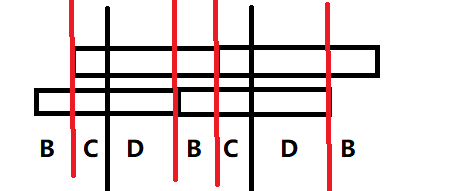
\includegraphics[width=7cm]{figure/p1.png}

        如上图所示，其中黑线表示倍数$ki$。上方的字符串的$A$就可以表示为$C+D+B$，下方字符串的$A$就可以表示为$B+C+D$。如果上方字符串$A+A$的左侧和右侧各接上一个相同的字符$a$，这就说明$B$的末尾为$a$，而上方字符串$A+A$的末尾也为$B$的末尾$a$，因此在$A+A$的末尾处就出现了长度为2的回文串。

因此对于跨过$ki$的可能的$A$只有一种时，可以通过后缀数组在$O(1)$的复杂度求出$S$的最长长度。

对于$S+t+A+A+rev(S)$、$S+A+t+A+rev(S)$、$S+A+A+t+rev(S)$这三种情况，可以通过类似的讨论来计算。

时间复杂度为$O(|t|\log |t|)$。
    \end{frame}

\begin{frame}
        \frametitle{\songti \bfseries K. Divisior Transformation}
        \begin{block}{\songti \bfseries 题意简述}

            给定 $1\sim n$ 的排列 $p$，有 $q$ 次询问：

            每次询问给定 $l,r,x$，枚举 $i=l\sim r$，若 $x|p_i$，则 $x=p_i/x$，若 $p_i|x$，则 $x=x/p_i$，否则不变。问最终$x$的值和中途 $p_i|x$ 或 $x|p_i$ 的次数。
            
            $n,m\le 10^6$
        \end{block}
    \end{frame}

    \begin{frame}
        \frametitle{\songti \bfseries K. Divisior Transformation}
        
        考虑以 $R$ 为右端点的询问和以 $R-1$ 为右端点的询问集合答案的差别，对于 $x|p_r$ 的，答案为 $x$ 的询问集合的答案会变为 $p_r/x$，对于 $x|p_r$ 的答案，答案为 $x$ 的询问集合的答案会变为 $p_r/x$，其他的答案不变。
        
        当 $x|p_r$ 时，$x$ 的答案变成 $p_r/x$，$p_r/x$的答案变成$x$。可以理解为答案为 $x$ 的集合和答案为 $p_r/x$ 的集合进行了交换。
        
        当 $p_r|x$ 时，可以理解为答案为 $x$ 的询问集合会和答案为 $x/p_r$ 的集合合并。
        
        合并可以用并查集来实现，这样就可以得到这题的做法，将询问离线，每次考虑将 $R$ 扩大，将 $l=R$ 的询问放入并查集中，查询 $r=R$ 的询问在并查集上的根，可以得到最终的 $x$。
        
        求中途 $p_i|x$ 或 $x|p_i$ 的次数，可以在并查集上打标记，利用带权并查集解决，枚举约数和倍数的复杂度为 $O(\sum \lfloor\frac{n}{i}\rfloor)=O(n\ln n)$，时间复杂度为 $O(n\log n+n\ln n)$
    \end{frame}

    \begin{frame}
        \frametitle{\songti \bfseries L. Larger or Smaller}
        \begin{block}{\songti \bfseries 题意简述}
        
            设 $f_{x,y}$ 表示有多少个 $1\sim n$ 的排列，$p_i<i$ 的位置的个数是 $x$ 且 $p_i>i$ 的位置的个数是 $y$。
            
            给定 $n$ 和模数 $m$，对所有合法的 $x,y$ 求 $f_{x,y}$。
            
            $n\le 2000.$
        \end{block}
    \end{frame}

        \begin{frame}
        \frametitle{\songti \bfseries L. Larger or Smaller}

            将 $i$ 看成点，$i$ 向 $p_i$ 连边，由于每个点只有一条入边，一条出边，因此最后的图会变成若干个环

            可以先单独考虑一个环的方案数，设 $g_{a,b}$ 表示一个大小为 $a+b$ 的环，$p_i<i$ 的个数为 $a$，$p_i>i $的个数为 $b$，这样的环的方案数。转移考虑新加入一个大于当前环上所有数的数，可以选择把这个数插入 $p_i<i$ 的边中，或者插入 $p_i>i$ 的边中，插入 $p_i<i$ 的边中，会增加一条 $p_i<i$ 的边，插入 $p_i>i$ 的边中，会增加一条 $p_i>i$ 的边，插入 $p_i<i$ 的边，会增加一条 $p_i<i$ 的边。
            
            因此可以得到$g_{a,b}=b\cdot g_{a-1,b}+a\cdot g_{a,b-1}$。
            
            在得到单个环的方案数后，一个办法是用 $O(n^3)$ 的时间，利用单个环的方案数 $dp$ 得到若干环的方案数。

但可以发现多个环可以一起考虑，只需要增加一个增加环的转移即可，具体就是加入一个最大的数，从$a+b-1$个数选择一个和最大数组合成环，于是可以得到$g_{a,b}=b\cdot g_{a-1,b}+a\cdot g_{a,b-1}+(a+b-1)\cdot g_{a-1,b-1}$

最后再考虑单个点的自环，直接利用组合数将单个点插入即可，即$f(n,x,y)=g_{x,y}\binom{n}{n-x-y}$，组合数可以利用$\binom{n}{m}=\binom{n-1}{m}+\binom{n-1}{m-1}$递推求得，时间复杂度为$O(n^2)$
    \end{frame}

   \begin{frame}
        \frametitle{\songti \bfseries M. Road2}
        \begin{block}{\songti \bfseries 题意简述}
给定一个无向图，每条边有边权，$f(u,v)$定义为$u$到$v$的最小瓶颈路，最小瓶颈路可以理解为只使用边权大于等于$x$的边，存在一条$u$到$v$的路径，最小的$x$即为$f(u,v)$

$q$组询问，询问$\sum_{i=l}^r\sum_{j=i+1}^rf(i,j)$

$n,q\le 50000,m\le 200000$
        \end{block}
    \end{frame}

    \begin{frame}
        \frametitle{\songti \bfseries M. Road2}
        
看出这是一个最小瓶颈路，于是使用kruscal重构树，暴力求解答案复杂度 $O(qn^2+m\log n)$。

对于每个点预处理答案，并处理成前缀和的形式，最后求答案时只用扫描一遍即可，复杂度 $O(qn+n^2+m\log n)$。

分析数据范围，想到分块预处理，对序列分块，每 $\sqrt{n}$ 个元素一块。
    \end{frame}

        \begin{frame}
        \frametitle{\songti \bfseries M. Road2}
        
第一步先对于每个点预处理出到每个块的答案和，这个可以对于每个块，进行一遍 dfs。把块内的点叫做关键点。dfs 的过程中存储当前点的子树内的任意点到所有子树外的关键点的答案的和。这一步的时空复杂度均为 $O(n\sqrt n)$。

第二步预处理两个块之间的答案，先对第一步得出的答案做一遍前缀和，然后扫一遍即可得出两块之间的答案，时间复杂度 $O(n\sqrt n)$，空间复杂度 $O(n)$。

第三步考虑查询时的散块与散块之间的贡献，这一步不能直接 dfs，考虑把关键点的虚树建出来然后再虚树上 dfs 即可。复杂度 $O(\sqrt{n})$。建虚树时使用排序算法复杂度可能会不正确，其实可以对于每一个块先排好序，然后再暴力扫这个块。 

于是我们就在时空复杂度均为 $O(n\sqrt n)$ 的复杂度下解决又这个题。其实只需要开一个 $O(n\sqrt{n})$ 的数组，所以不知道空间会不会很卡。
    \end{frame}

    \begin{frame}
        \frametitle{致谢}
        感谢 ACMM 学术部为比赛题目的付出。

        感谢 Codeforces 提供的 polygon 平台。

        感谢深圳中学 OI 队赛前帮忙验题。
    \end{frame}

\end{document}